\chapter{Organizzare l'insegnamento}
\label{cha:intro}
Per trasmettere ad altri le proprie conoscenze e abilità e quindi fare in modo che l'insegnamento abbia successo bisogna creare un programma o percorso di studio. Per strutturare il programma in modo efficace è fondamentale completare tre passaggi, di cui due preliminari alla programmazione vera e propria.\\
Il primo passo è individuare gli obiettivi di insegnamento per mettere a fuoco temi e contenuto di ciò che verrà insegnato, tenendo ben presente anche il livello di attitudine che si vuole raggiungere del tema affrontato. È in questa fase che andremo ad utilizzare la Tassonomia di Bloom, uno strumento di analisi che ci permette di esaminare i diversi gradi di familiarità che si possono raggiungere con un determinato tema.\\
Il secondo passo è la comprensione di chi ci sta davanti. Per riuscire a trasmettere informazioni in modo efficace dobbiamo prima di tutto capire come la persona che riceverà l'insegnamento preferisce che le informazioni gli vengano presentate.\\
Il terzo passaggio è, appunto, la programmazione del percorso didattico, momento in cui le lezioni vengono organizzate e in cui vengono registrati i risultati ottenuti.
\section{Individuare gli obiettivi di insegnamento}
\label{sec:context}
Per posare le basi di un buon insegnamento bisogna innanzitutto fissare dei buoni obiettivi di insegnamento.
La tassonomia di Bloom è una classificazione dei diversi obiettivi da raggiungere attraverso l'istruzione formale condotta da Benjamin Bloom nel 1948 sulla base di tre aspetti utilizzati per stabilire un consenso sugli obiettivi dell'educazione: cognizione, affettività e psicomotricità. Si tratta di una classificazione degli obiettivi effettuata in modo gerarchico, organizzata sulla base del fatto che l'attività richieda un'elaborazione più o meno complessa.


\begin{figure}[h!]
  \centerline{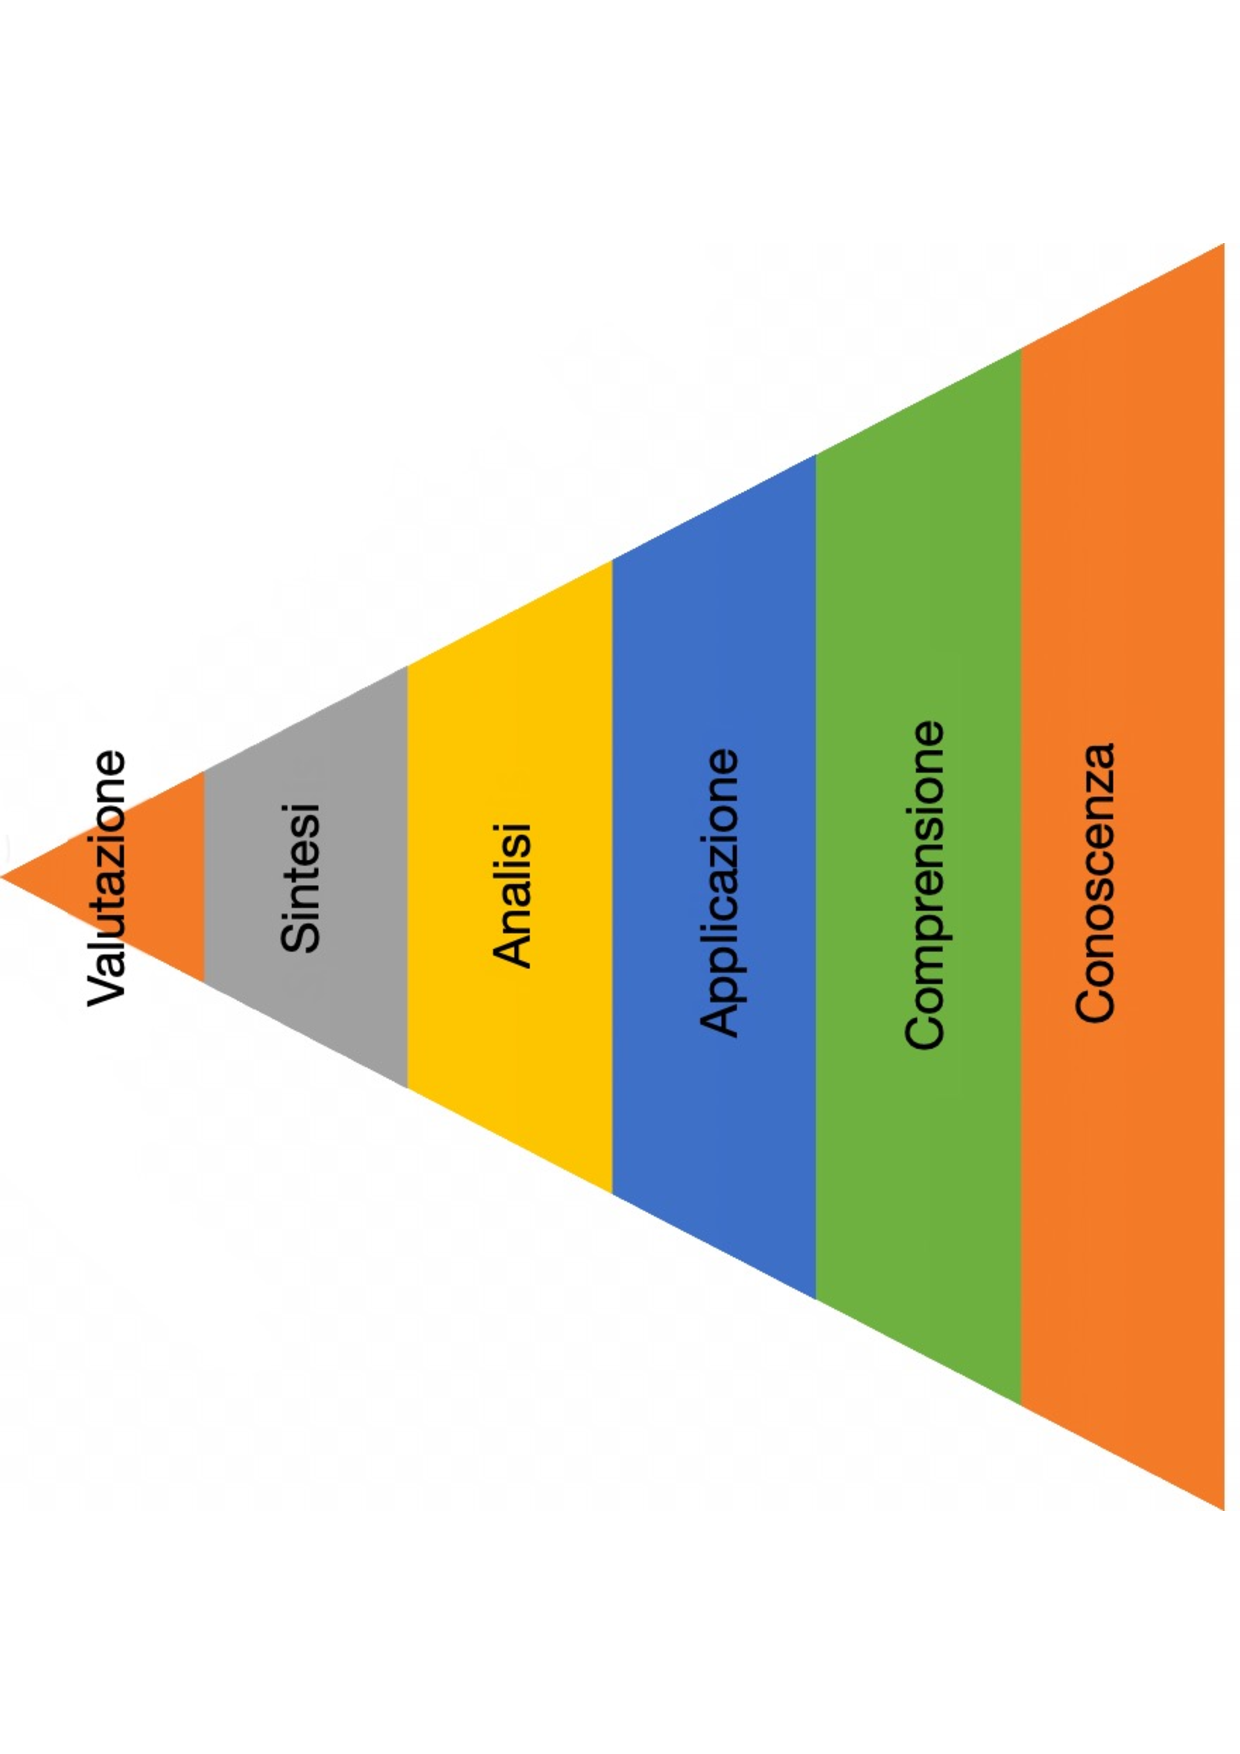
\includegraphics[height = 9 cm, width= 6 cm, angle=270]{figures/bloom.pdf}}
  \caption{Piramide di Bloom}
\end{figure}
\begin{itemize}
  \item La \textbf{conoscenza} è l'abilità cognitiva fondamentale e si riferisce alla memorizzazione di informazioni specifiche e discrete, come fatti e definizioni o metodologie.  La conoscenza può essere valutata con mezzi semplici, ad esempio con domande a scelta multipla o a risposta breve che richiedono il recupero o il riconoscimento di informazioni.

  \item La \textbf{comprensione} viene dimostrata dagli studenti che parafrasano le informazioni che incontrano con parole proprie, classificando gli elementi in gruppi, confrontando e contrastando gli elementi con altre entità simili o spiegando un principio ad altri.

  \item L'\textbf{applicazione} delle conoscenze, delle abilità o delle tecniche in nuove situazioni indicano il grado di competenza dello studente nel terzo livello della tassonomia di Bloom. Un esempio di applicazione familiare ai bibliotecari medici è la capacità di utilizzare le migliori pratiche nel processo di ricerca della letteratura, come l'uso dei termini MeSH (Medical Subject Headings) per i concetti chiave di una ricerca.

  \item L'\textbf{analisi} di un concetto dimostra l'abilità nella formulazione di un pensiero critico. La distinzione tra fatti e opinioni e l'identificazione delle affermazioni su cui si basa un'argomentazione richiedono un'analisi. Così come la scomposizione di un bisogno informativo nelle sue componenti per identificare i termini di ricerca più appropriati.  L'uso di questo livello è potenzialmente confuso e spesso produce imprecisioni. Alcuni educatori praticanti possono "analizzare" le informazioni ottenute piuttosto che valutare criticamente le conoscenze in termini di validità e accuratezza delle prove. L'analisi della qualità delle conoscenze viene confusa con l'analisi del problema. L'analisi è la valutazione critica delle conoscenze.

  \item Il livello di \textbf{sintesi} comporta la creazione di un prodotto nuovo in una situazione specifica. Un altro esempio riguardante il mondo medico basata sulle evidenze che richiede una sintesi è la formulazione di un quesito clinico ben costruito dopo aver analizzato le lacune informative di un medico.

  \item La \textbf{valutazione} è importante per la formulazione di pensieri critici. Un esempio di questo potrebbe essere quando gli insegnanti riflettono su una sessione di insegnamento e utilizzano il feedback dei partecipanti e i risultati della loro valutazione per giudicare il valore della propria sessione.
\end{itemize}
Sulla base delle scoperte della scienza cognitiva successive alla pubblicazione originale, una successiva revisione della tassonomia modifica la nomenclatura e l'ordine dei processi cognitivi della versione originale. In questa versione successiva, i livelli sono: ricordare, comprendere, applicare, analizzare, valutare e creare.
\begin{figure}[h!]
  \centerline{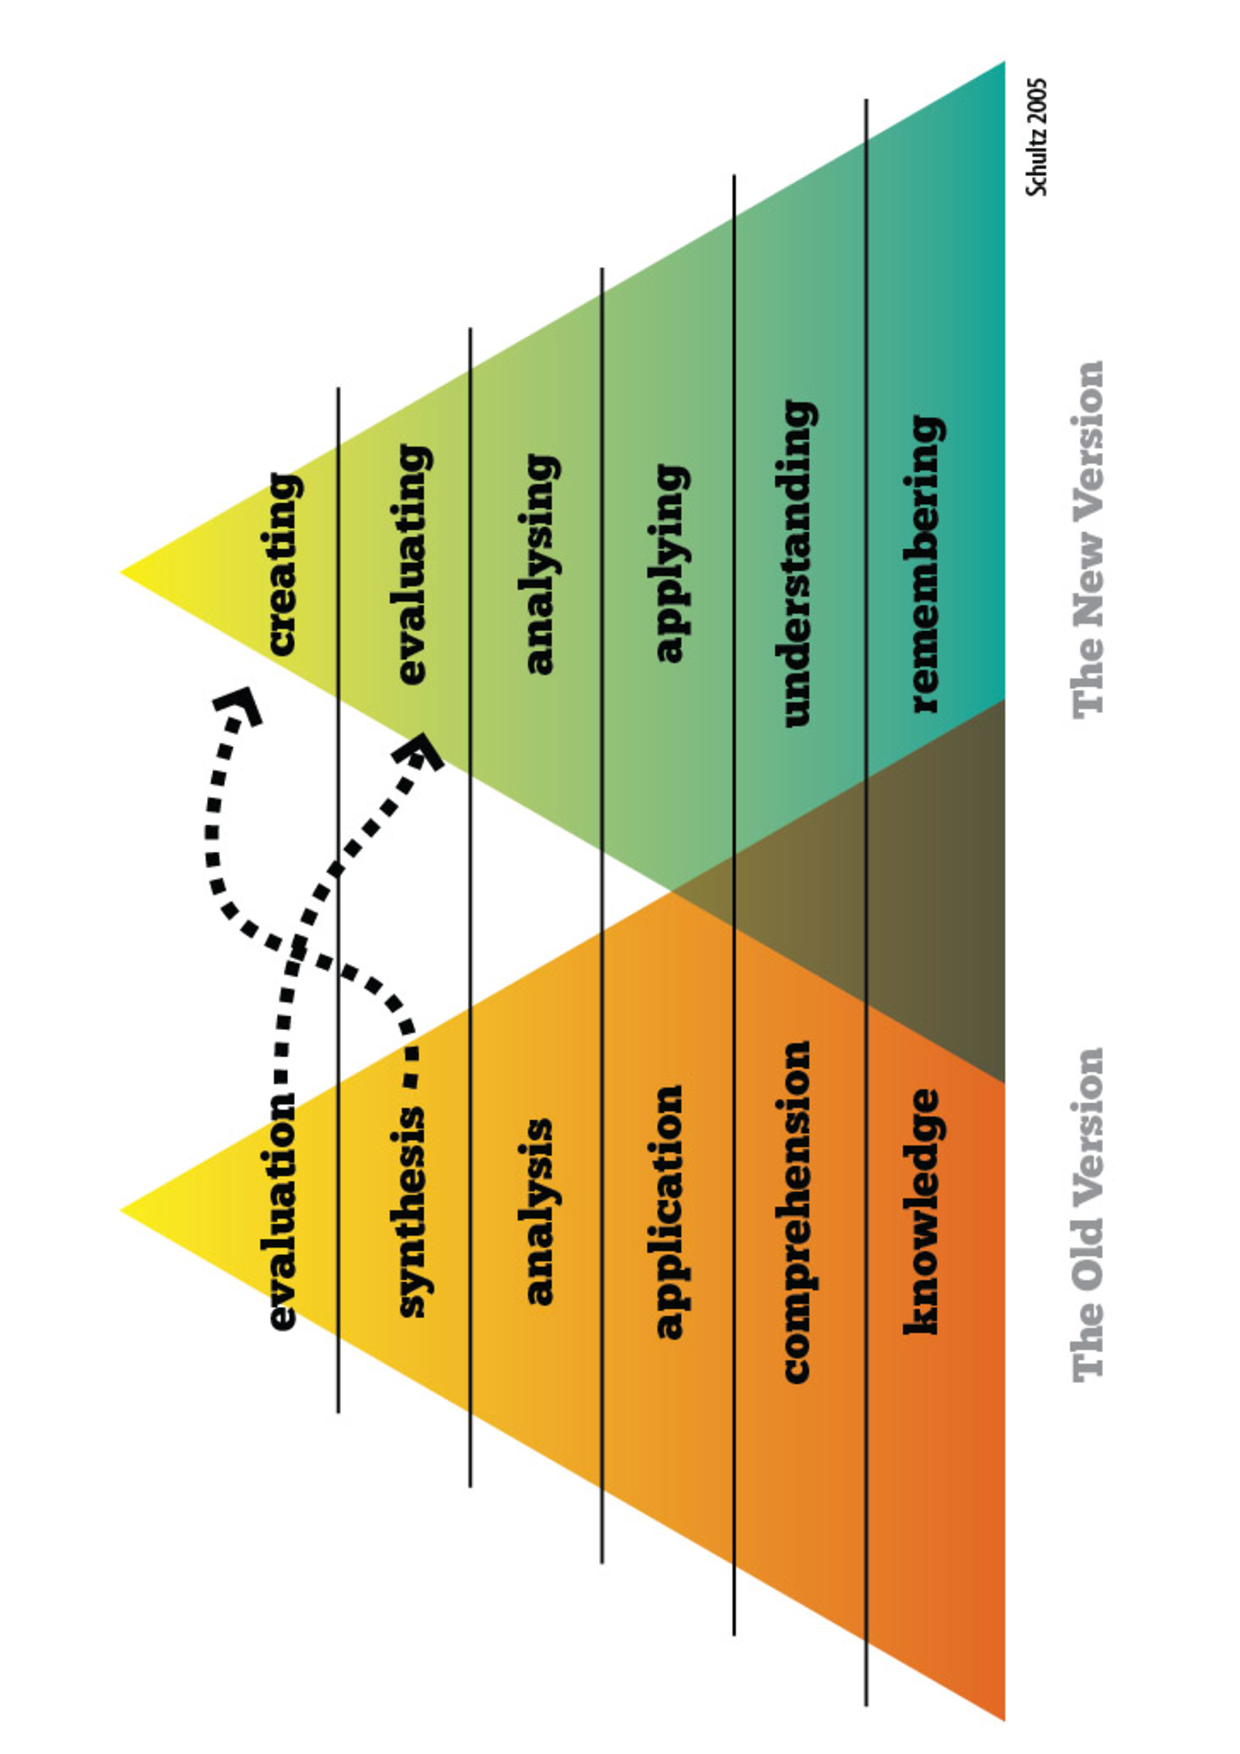
\includegraphics[height = 9 cm, width= 6 cm, angle=270]{figures/BloomNew.pdf}}
  \caption{Piramide di Bloom}
\end{figure}
Questa revisione aggiunge una nuova dimensione a tutti e sei i processi cognitivi. Specifica i quattro tipi di conoscenza che potrebbero essere affrontati da un'attività di apprendimento: fattuale (terminologia e fatti discreti); concettuale (categorie, teorie, principi e modelli); procedurale (conoscenza di una tecnica, di un processo o di una metodologia); e metacognitiva (che comprende la capacità di autovalutazione e la conoscenza di varie abilità e tecniche di apprendimento).

\subsection{Applicazione della Tassonomia di Bloom}
Di seguito sono riportati alcuni esempi per il raggiungimento di specifici learning goals utilizzando l’approccio della tassonomia di Bloom in vari campi di studio.
\\
\\


\begin{itemize}
\item Esempio uno - Applicazione in campo medico, gli shock\\
\\
Tipicamente programmi didattici e le valutazioni si concentrano spesso sull'acquisizione di conoscenze che mirano ai livelli inferiori della tassonomia di Bloom. Gli educatori insegnano comunemente ai livelli inferiori della tassonomia di Bloom, ricordare e capire. Gli educatori clinici di medicina invece dovrebbero sfruttare i livelli più alti dell'apprendimento cognitivo piuttosto che limitarsi a ricordare e richiamare le conoscenze. La qualità dell'apprendimento nella formazione medica potrebbe essere compromessa senza puntare ai livelli cognitivi più alti della tassonomia. Per facilitare questa applicazione, gli educatori dovrebbero avere a disposizione esempi clinici semplificati di ogni specialità. Inoltre, l'uso di scenari clinici pratici ed esercizi consentirà agli educatori di familiarizzare con la tassonomia e di utilizzarla e applicarla in modo più ampio, portando a una valutazione complessivamente migliore.\\
  \\
Primo livello: Memorizzare la definizione di shock, i criteri clinici, le sue classi, test diagnostici per lo shock, i farmaci e gli interventi comunemente utilizzati. \\
Secondo livello: Comprendere lo spettro della presentazione clinica, classificando i tipi di shock e la loro relazione con la causa sottostante come ad esempio i cambiamenti dei segni vitali.\\
Terzo livello: Applicare le conoscenze per diagnosticare la condizione ed eseguire le misure di rianimazione specifiche per ogni tipo di shock.\\
Quarto livello: Analizzare le evidenze relative ai migliori approcci terapeutici in vari contesti e differenziare i diversi stati di shock in base agli endpoint clinici ed emodinamici.\\
Quinto livello: Valutare la validità del monitoraggio invasivo e il suo effetto sugli esiti o le differenze tra i tipi di fluidi per la rianimazione.\\
Sesto livello: Creare o innovare nuove conoscenze, come la convalida di nuove misure diagnostiche o di nuovi marcatori prognostici.\\
\\
\item Esempio due - Applicazione in ingegneria del software\\
\\
Primo livello: Le domande sul livello di conoscenza includono le parole chiave definire, elencare, organizzare, ordinare e dichiarare.
Di seguito sono riportati alcuni esempi di domande che rientrano in questo livello:
Che cos'è una variabile globale?
Elencare 5 parole riservate nella programmazione C.
Indicare quattro attributi di un software ben progettato.
Definire quattro tipi di tracciabilità.\\
\\
Secondo livello: Identificare il valore di x dopo aver eseguito questo frammento di programma:
\begin{lstlisting}
  x=0; y=0;
while (y<50) {
   x++; y=y+5
}
  \end{lstlisting}

Prevedere l'output di questo frammento di programma:

\begin{lstlisting}
  i=0;
  while (i<=10) {
     printf(“\%3d \%3d\n”, i, 50–i);
     i++;
  }
  \end{lstlisting}
  Descrivete i 4 tipi di accoppiamento nella progettazione del software.
  Descrivete il principio di Pareto nell'assicurazione statistica della qualità del software.\\
  \\
  Terzo livello: Scrivere un ciclo for che produca questo output:

  \begin{lstlisting}
    0  1
    1  2
    2  4
    3  8
    4  16
    5  32
    6  64
    \end{lstlisting}

    Scrivere un'istruzione if per calcolare e visualizzare la media di un insieme di n numeri. Il calcolo deve essere eseguito solo se n è maggiore di 0, altrimenti deve essere visualizzato un messaggio di errore.\\
    Sviluppo di un sistema software per l'azienda XYZ. Il cliente non è sicuro di come dovrebbe essere il sistema finale. Quale modello di sviluppo software sarebbe adatto a questo progetto? Giustificate la scelta del modello di sviluppo del software.\\
    Dati i seguenti requisiti, classificarli come requisiti funzionali o non funzionali: sicurezza, funzione per calcolare il costo di un articolo in base alla politica di sconto corrente, affidabilità.\\
    Quarto livello: Le domande del livello di analisi includono le parole chiave: analizzare, confrontare, contrastare, distinguere, categorizzare, calcolare e testare.\\
    Distinguere tra call by value e call by reference.\\
    Distinguere le chiamate alla funzione printf per la visualizzazione di messaggi e per l'eco dei dati.\\
    Dato un un team democratico di cinque membri, calcolare il numero di vie di comunicazione necessarie.\\
    Confrontate e contrastate il modello a cascata con il modello di prototipazione.\\
    \\
    Quinto livello: Le domande del livello di sintesi includono le parole chiave creare, costruire, progettare, sviluppare, gestire, organizzare, pianificare, prevedere e proporre.\\
    Costruire un programma C completo che legga stringhe di testo da un file di testo in una struttura dati adeguata, ordini l'elenco in ordine crescente, lo visualizzi sullo schermo e lo memorizzi in ordine nel file di testo. Giustificate la scelta della struttura dati.\\
    Scrivete un programma C che accetti input interi dallo schermo, calcoli i valori totali e medi ne visualizzi i valori.\\
    Progettare l'architettura del sistema software sulla base dei requisiti definiti nel documento Software Requirement Specification.\\
    \\
    Sesto livello: Le domande del livello di valutazione includono le parole chiave argomentare, discutere, raccomandare, dare priorità, giustificare, valutare e decidere.
    Date le due soluzioni al problema di programmazione indicato, valutare le soluzioni in termini di efficienza e leggibilità.\\
    Quale dei due algoritmi, bubblesort o quicksort, è più efficiente? Giustificate la risposta.\\
    Date due possibili soluzioni, A e B, per risolvere il problema di sviluppo software indicato, decidete la soluzione migliore fornendo la propria giustificazione.\\
    Dati tre possibili approcci per implementare il sistema definito, discutete i possibili vantaggi e svantaggi di ciascuno.

\item Esempio tre - Applicazione in campo letterale\\
\\
Utilizzando la Tassonomia revisionata è stato presentato un obiettivo di lezione basato sulla storia di "Riccioli d'oro e i tre orsi" per ciascuno dei sei livelli del processo cognitivo.\\
\\
Primo livello: Descrivere dove viveva Riccioli d'oro.\\
Secondo livello: Riassumere il significato della storia di Riccioli d'Oro.\\
Terzo livello: Costruire una teoria sul perché Riccioli d'oro sia entrato nella casa.\\
Quarto livello: Differenziare il modo in cui Riccioli d'Oro ha reagito rispetto a come avreste reagito voi in un evento simile.\\
Quinto livello: Comporre una canzone, una scenetta, una poesia per trasmettere la storia di Riccioli d'oro in una nuova forma.\\
Sesto livello: Valutare se si pensa che sia successo davvero a Riccioli d'Oro.
\end{itemize}
\section{Strategie di apprendimento}
\label{sec:problem}

Una volta definiti i \textit{learning objectives} è il momento di decidere come questi verranno raggiunti. In un contesto educativo con molta probabilità l'insegnamento è rivolto verso una classe. Una classe è un gruppo eterogeneo di persone ed proprio questa caratteristica di eterogeneità l'aspetto più arduo da dover affrontare. Ogni studente ha il proprio modo di imparare concetti nuovi in base al proprio \textbf{stile di apprendimento} è quindi importante distinguere e riconoscere gli stili di ogni stuente per così aggevolare l'apprendimento di esso, in quanto l'intervento sugli stili è inscindibile da quello sulle strategie di apprendimento.

\subsection{Stili di apprendimento}
Con questo termine si indica \textit{"l'approccio all’apprendimento preferito di una persona, il suo modo tipico e stabile di percepire, elaborare, immagazzinare e recuperare le informazioni”} (Mariani, 2000).
Uno stile di apprendimento è descrittivo delle tendenze di una persona in continua evoluzione. Non incasellano l'individuo in tipi astratti ma ne descrivono la complessità e l'unicità di essa. Per definirne uno occorre ragionare su tre variabili:

\begin{itemize}
  \item \textbf{Preferenze ambientali} a loro volta definite da: luogo di studio che potrebbe essere casa o la biblioteca. Dall'orario preferito. Dalla preferenza di studiare in compagnia o da soli. Oltre ad altri fattori minori come l'illuminazione, suoni che possono essere rumori di sottofondo oppure musica o la preferenza del silenzio. Consumi alimentari, se si è abituati a consumare cibi o bevande durante lo studio.
  \item \textbf{Stili cognitivi} che intende la \textit{“modalità di elaborazione dell’informazione che la persona adotta in modo prevalente, che permane nel tempo e si generalizza a compiti diversi”} (Boscolo, 1981).
  Lo stile cognitivo demarca tre fattori: il modo in cui vengono percepiti i fenomeni, le procedure razionali dell'individuo e la modalità di memorizzazione e organizzazione dello studio.
  La percezione può essere analitica o globale a seconda se ci si sofferma prima sui dettagli o alla creazione di una visione d'insieme.
  La memoria può essere verbale o visiva in base alla preferenza di ricezione delle informazioni che possono essere sotto forma di libri o di una spiegazione.
  Il ragionamento si descrive con una coppie di aggettivi. Il primo è una scelta tra sistematico, che caratterizza un approccio a piccoli passi, o intuitivo quando vengono definite regole generali sempre valide. Il secondo aggettivo può essere impulsivo oppure riflessivo, questi indicano la velocità con la quale si traggono conclusioni.
  \item \textbf{Modalità sensoriale} che sono raggruppabili in quattro gruppi. Il primo gruppo è rappresentato dal canale Visivo verbale, quello che passa di preferenza per la letto-scrittura. Il secondo gruppo è rappresentato dal canale Visivo iconografico, ovvero la preferenza per immagini, disegni, fotografie, simboli, mappe concettuali, grafici e diagrammi. Il terzo gruppo è rappresentato dal canale Uditivo, ovvero la preferenza per l’ascolto. Le informazioni vengono assorbite maggiormente assistendo ad una lezione, partecipando a discussioni e attraverso il lavoro con un compagno o a gruppi. Il quarto gruppo è rappresentato dal canale Cinestetico, ovvero la preferenza per attività concrete.
\end{itemize}
Vale la pensa soffermarsi du questa ultima variabile, in quanto fondamentale per capire quali elementi non devono mancare in un programma di apprendimento con gamification ben congegnato.
\subsection{Cono dell'esperienza di Dale}

\begin{figure}[h!]
  \centerline{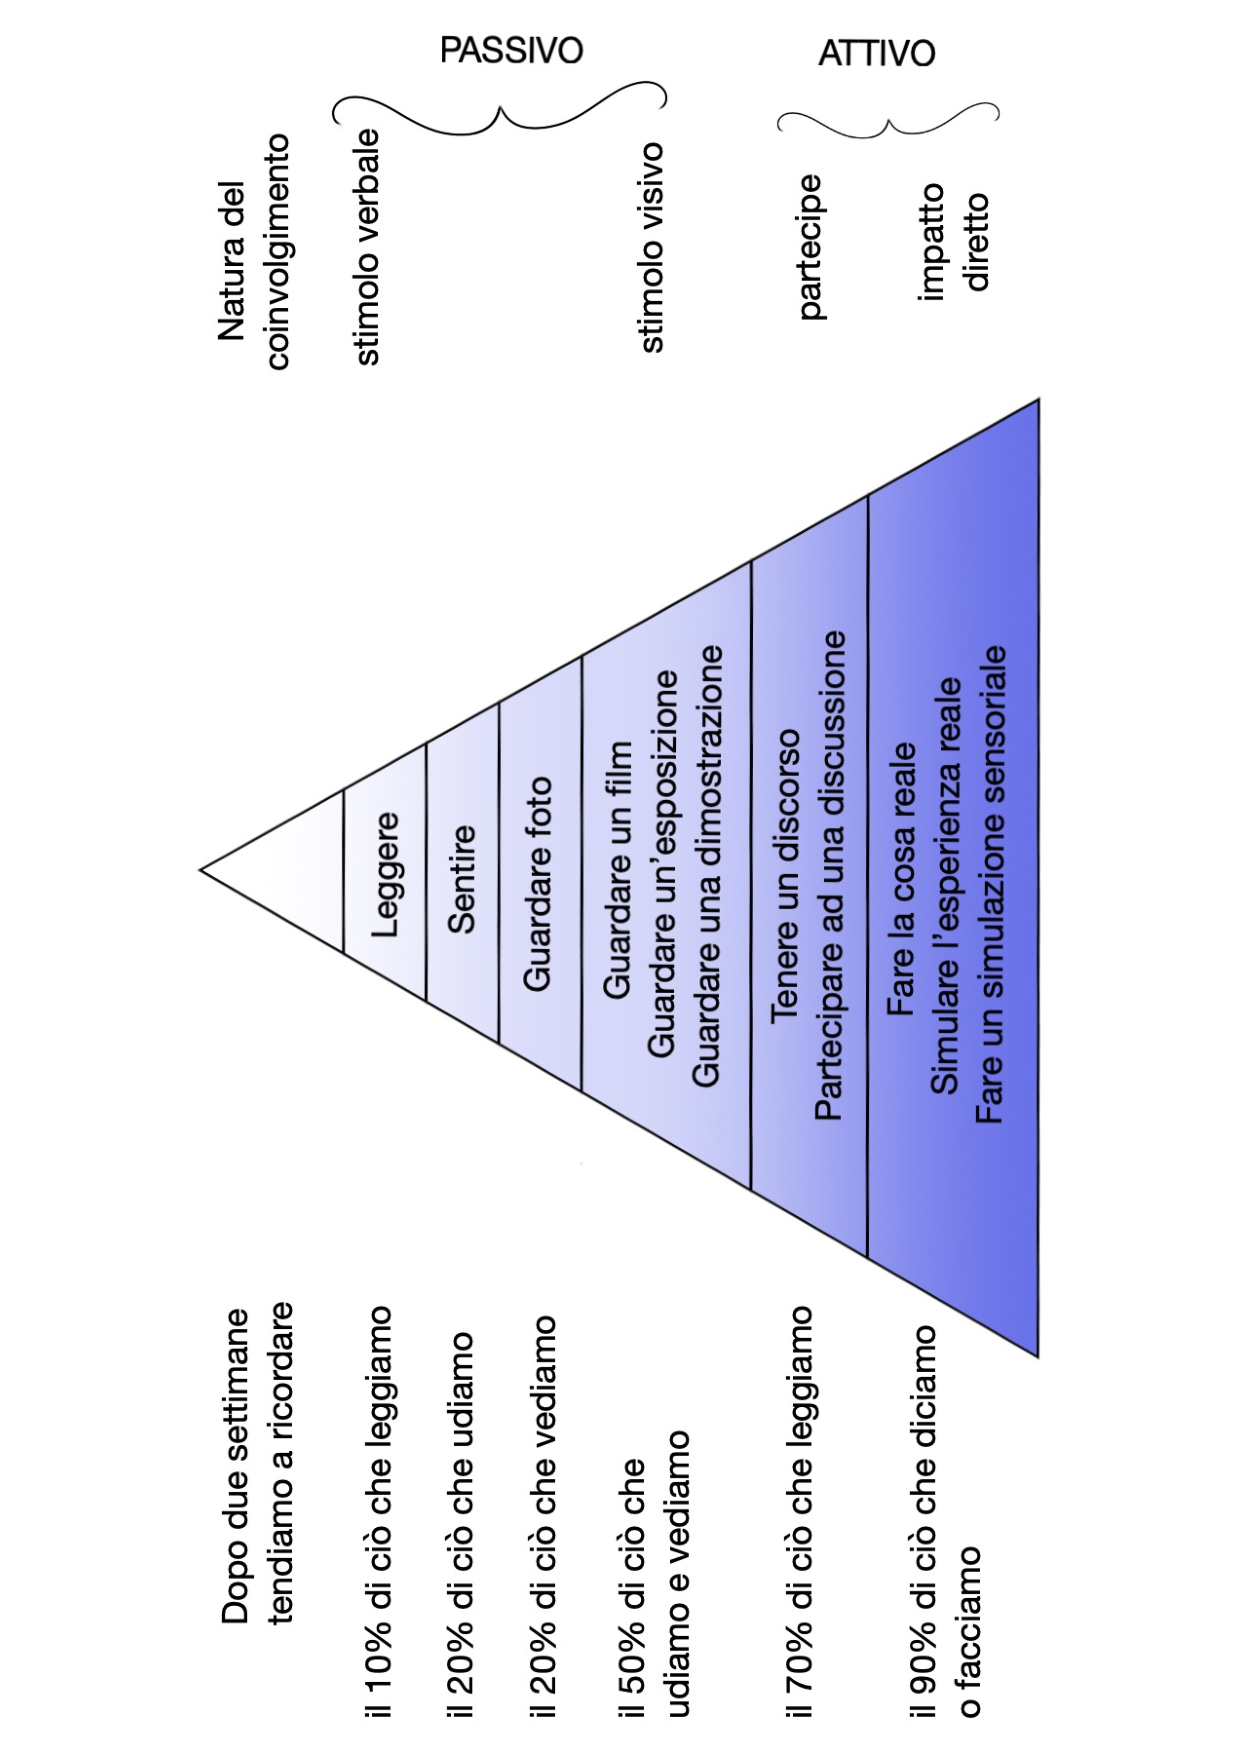
\includegraphics[height = 12 cm, width= 8 cm, angle=270]{figures/cono.pdf}}
  \caption{Cono dell'apprendimento, Edgar Dale, 1969.}
\end{figure}
Nel 1946, Edgar Dale introdusse il Cono dell'Esperienza, dove vengono raffigurati in prograssione dall'alto verso il basso tutti i tipi di esperienza dalla più astratta alla più concreta. Il Cono dell'Esperienza si propone di informare i lettori su quanto le persone ricordano in base al modo in cui incontrano le informazioni. Secondo la ricerca il metodo meno efficace di insegnamento prevede l'apprendimento di informazioni presentate attraverso simboli verbali, ovvero la lettura e l'ascolto di parole. Il metodo più efficace prevede esperienze di apprendimento dirette e mirate, come lavori di laboratorio e prove più simili possibile alla realtà e all'esperienza diretta sul campo. Il Cono di Dale rivela che le tecniche "action-learning" consentono una ritenzione fino al 90\% delle informazioni.\\
\\
Potrebbe sembrare che il principio alla base della teoria di Dale sia in contrasto con la diversità degli stili di apprendimento possibili, di cui si parlava nel paragrafo precedente. in realtà però non si tratta di una "gerarchia", in cui uno stile è superiore a un altro, ma dell'importanza di prevedere una combinazione di stimoli sensoriali diversi che permettano un assorbimento più efficace delle informazioni. In sostanza, leggere una nozione su un libro (stimolo visivo verbale), sentirla spiagare a lezione da un professore, magari con il supporto di slide (stimolo uditivo verbale + stimolo iconografico e parlarne con dei compagni di studio (partecipazione) è chiaramente più efficace che limitarsi a leggerla.
\\
Le persone imparano meglio quando utilizzano stili di apprendimento percettivi. Questi sono basati sulla sensorialità. Più canali sensoriali sono possibili nell'interazione con una risorsa, maggiore è la possibilità che molti studenti possano imparare da essa. Secondo Dale, gli insegnanti dovrebbero progettare attività didattiche che si basino su esperienze di vita reale.
Il cono dell'esperienza è uno strumento che aiuta gli insegnanti a prendere decisioni sulle risorse e sulle attività. L'istruttore può chiedersi quanto segue:
\begin{itemize}
  \item Dove si collocherà l'esperienza dello studente con questa risorsa didattica nel cono?
  \item Quanto è lontana dalla vita reale?
  \item Che tipo di esperienza di apprendimento si vuole fornire in classe?
  \item In che modo questa risorsa didattica aumenta le informazioni fornite dal libro di testo?
  \item Quali e quanti sensi possono essere utilizzati dagli studenti per apprendere questo materiale didattico?
  \item Il materiale didattico migliora l'apprendimento?
\end{itemize}
\section{Creazione di un piano didattico}
\label{sec:problem}
Un piano didattico aiuta a rendere l'insegnamento più soddisfacente e meno dispendioso in termini di tempo. Aiuta l'istruttore a pianificare ciò che gli studenti devono imparare e a rendere l'insegnamento efficace. Strutturare obiettivi predefiniti e appropriati per ogni sessione didattica migliora i risultati dell'apprendimento e consente di misurare gli obiettivi. Un piano didattico dovrebbe contenere le seguenti specifiche, come riportato qui di seguito.
\begin{figure}[h!]
  \centerline{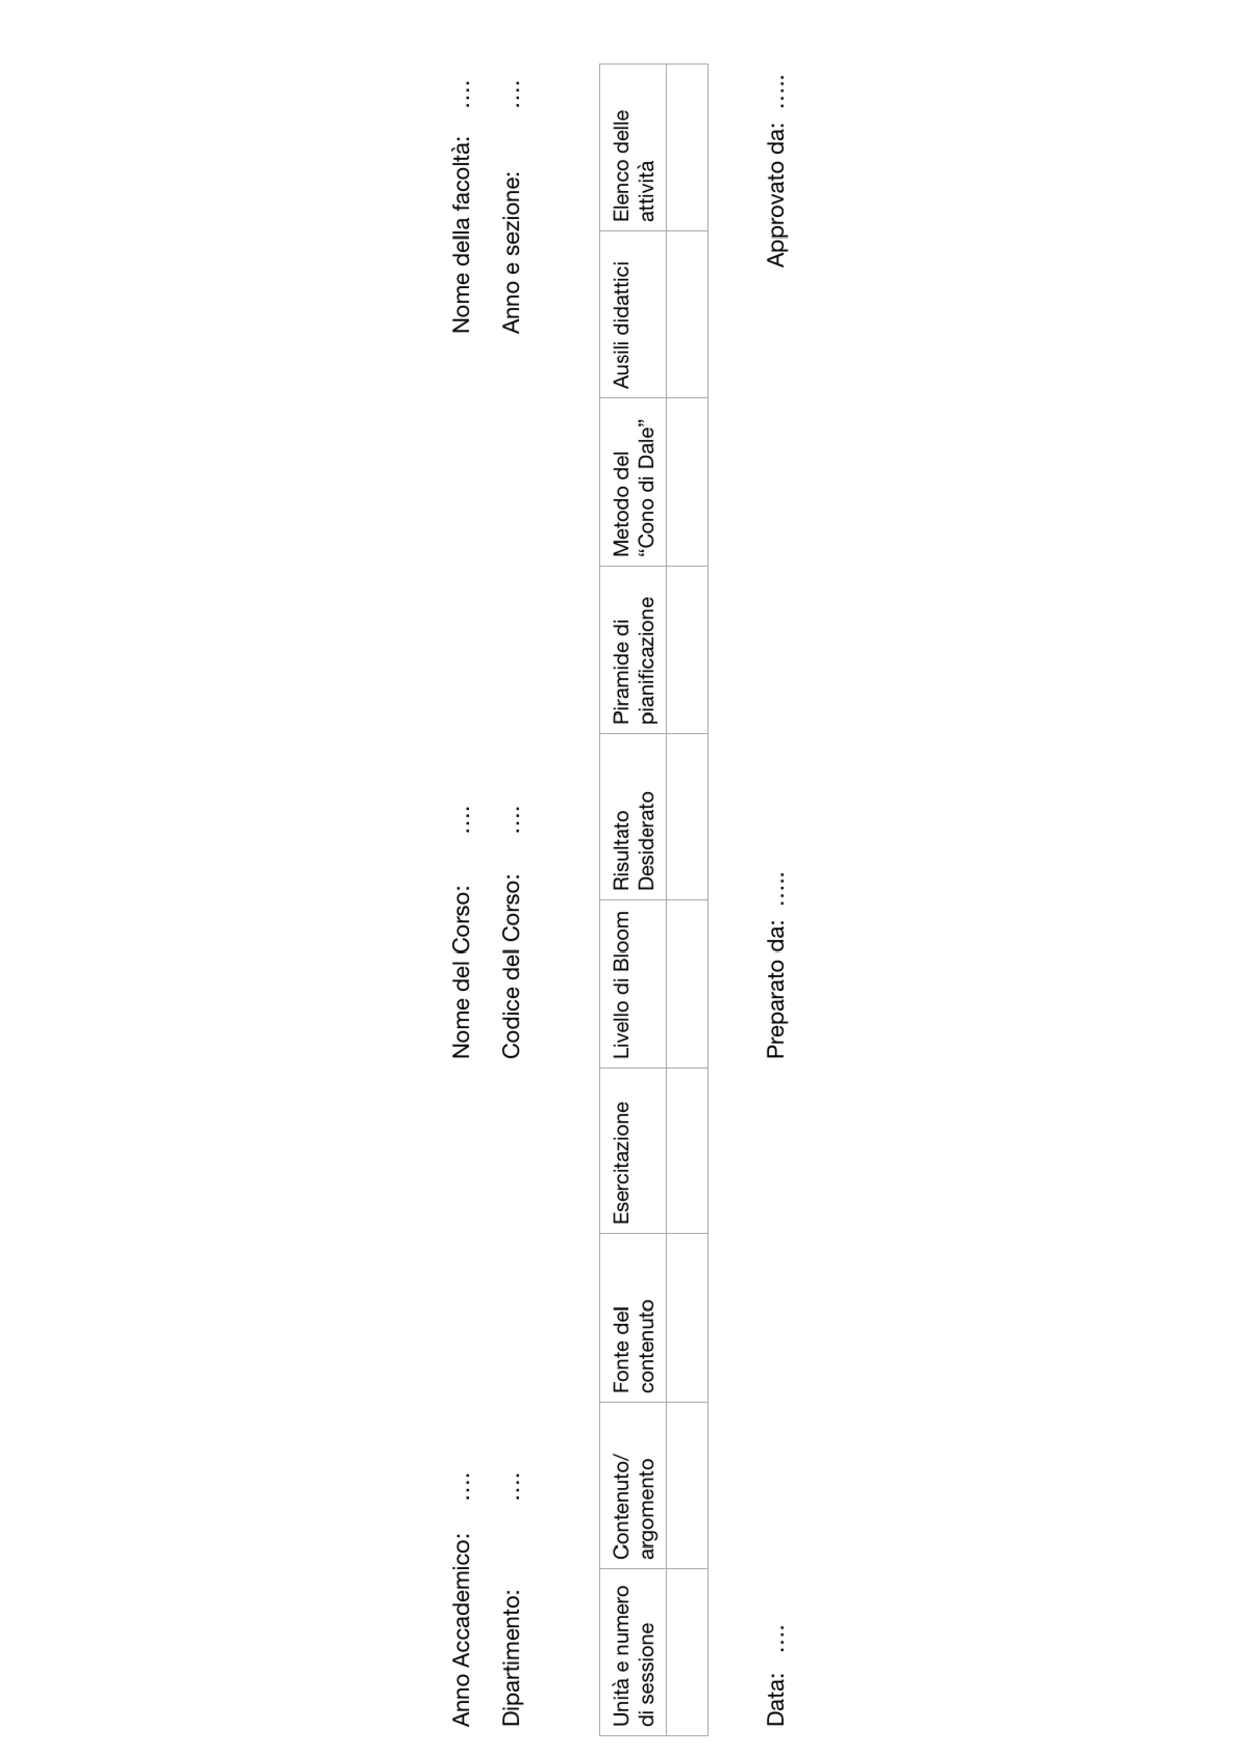
\includegraphics[height = 17 cm, width= 5 cm, angle=270, trim= 7cm 0 7cm 0]{figures/piano.pdf}}
  \caption{Esempio di piano didattico}
\end{figure}

I campi principali del piano sono i seguenti:
\begin{itemize}

\item Unità e numero di sessione: tiene conto delle ore totali assegnate all'argomento.
\item Contenuto/argomento: Specifica il nome dell'argomento che verrà trattato nella sessione corrispondente.
\item Fonte del contenuto: Specifica il libro di riferimento, i manuali e altro materiale di cui il contenuto è stato preparato.
\item Esercitazione: Meccanismo di riflessione per la comprensione del discente.
\item Livello di Bloom: Specifica a quale livello della tassonomia di Bloom è rivolto il corso.
\item Risultato del corso: Specifica l'apprendimento significativo che gli studenti hanno raggiunto.
\item Piramide di pianificazione: Aiuta a pianificare i contenuti per le diverse categorie di studenti. Ha tre livelli: ciò che tutti gli studenti imparano, ciò che la maggior parte degli studenti imparerà e ciò che alcuni studenti impareranno.

\item Dale's cone method: Specifica il metodo di apprendimento attivo, ad esempio leggere, ascoltare parole, guardare immagini, partecipare a una discussione, ecc.
\item Ausili didattici: Specifica strumenti come supporti visivi e presentazioni interattive per rendere l'esperienza di apprendimento interessante per gli studenti.
\item Elenco delle attività: Specifica attività come giochi di ruolo e demo di prototipi per il contenuto.
\end{itemize}
Ogni corso avrà un contenuto con caratteristiche adeguate. Ogni contenuto ha un obiettivo per alcuni livelli selettivi della Tassonomia di Bloom. L'esperienza reale nella simulazione dei concetti secondo il cono di Dale aiuta il discente a comprendere facilmente contenuti complessi.

\section{Impostazione di una valutazione}
\label{sec:problem}
L'impostazione della valutazione è raccomandato agli educatori per trovare un equilibrio impostando un foglio di domande che verifichi sia le abilità di pensiero di ordine inferiore sia quelle di ordine superiore degli studenti.
È stato introdotto il seguente modello (LO/IO/HO) per consentire al personale di applicare i concetti durante l'elaborazione delle domande.\\
LO - LOCQ - Domande cognitive di ordine inferiore. Verifica memoria e comprensione.\\
IO - IOCQ - Domande cognitive di ordine intermedio. Verifica applicazione e analisi.\\
HO - HOCQ - Domande cognitive di ordine superiore. Verifica valutazione e creazione.\\
\\
Nella seguente tabella sono riportati alcuni esempi di applicazione della tassonomia di Blooms nell'impostazione di alcune domande tipiche:\\
\\
\begin{tabular}{|l|l|l|r|}
  \hline
  n & Domanda & Classificazione \\
  \hline
  1 & Definire la legge di Ohm & LO(LOCQ)\\
  \hline
  2 & Qual è il valore quadratico medio di una corrente alternata? & LO(LOCQ) \\
  \hline
  3 & Classificare i suoli in base ai dati forniti & IO((IOCQ)\\
  \hline
  4 & Progettare un circuito pneumatico per l'applicazione descritta & HO(HOCQ)\\
  \hline
  \end{tabular}\\
\\
\\
Piontek nel 2008 in una pubblicazione dell'Università del Michigan, afferma che gli studenti dovrebbero sentire che il documento di valutazione sia equo e significativo. I dati di valutazione, che riflettono i risultati degli studenti, dovrebbero supportare questo fatto.
Nel processo di impostazione dei questionari si consiglia all’educatore di fornire i dettagli della distribuzione dei punteggi totali tra le domande LO/IO/HO del documento. La tabella seguente mostra, a titolo di esempio, la distribuzione percentuale dei voti in un caso possibile.\\
\\
\begin{tabular}{|l|l|l|r|}
  \hline
  Livello di cognizione & LO(LOCQ) & IO((IOCQ) & HO(HOCQ) \\
  \hline
  Distribuzione di voto raccomandata & 20 - 30\% & 40 - 50\% & 30 - 40\%\\
  \hline
  \end{tabular}\\
\\
La questione del bilanciamento della distribuzione dei punteggi tra LO/IO/HO è normalmente lasciata al personale che prepara il documento.
In questo metodo, si ritiene che le domande mettano alla prova le capacità di analisi, progettazione e pensiero critico degli studenti, oltre alla loro comprensione di base dell'argomento.
In un articolo sulla "Valutazione per l'apprendimento", Brown nel 2004, 2005 sottolinea che i criteri di valutazione devono essere chiari, espliciti, formulati in un linguaggio significativo per il personale e gli studenti e disponibili. Questo deve essere coerente a tutti i livelli degli anni di studio.\\
\\
È necessario menzionare che l'applicazione della tassonomia di Bloom deve riguardare i risultati di apprendimento del modulo da testare. Nusche nel 2008 ha affermato con forza che i risultati dell'apprendimento dovrebbero costituire la base di qualsiasi tipo di valutazione.
La distribuzione dei punteggi in base alla classificazione LO/IO/HO dipende anche dall'anno di studio per il quale viene preparato il questionario. Inoltre, anche il tipo di modulo, che può essere analitico o teorico, gioca un ruolo nella distribuzione appropriata delle domande tra i diversi livelli cognitivi.
Va anche detto che i principi della tassonomia di Bloom servono come linee guida per il personale che prepara il questionario, ma è in gran parte lasciato a loro il compito di produrre un documento equilibrato come risultato finale.
\\
\\
\\
\\
\\
\\
\\
\\
\\
\\
\\
\\
\\
\\
